% I am generally not editing this section - mainly focusing on questions and feedback - since it isn't done.

\section{Computational Setup}
% I'm not quite following this introduction para
Figure \ref{fig:ETAFLOW} displays the research approach methodology with a primary focus on the original ETA. 
The work performed previously has a completed design for the original ETA. 
The enhanced fission product ETA and ETA-SPNS will have objective spectra from referenced sources. 
The computational flow requires a baseline ETA design to use Coeus. 
Each of the computational steps is explained further below. 

\begin{figure}[ht]
	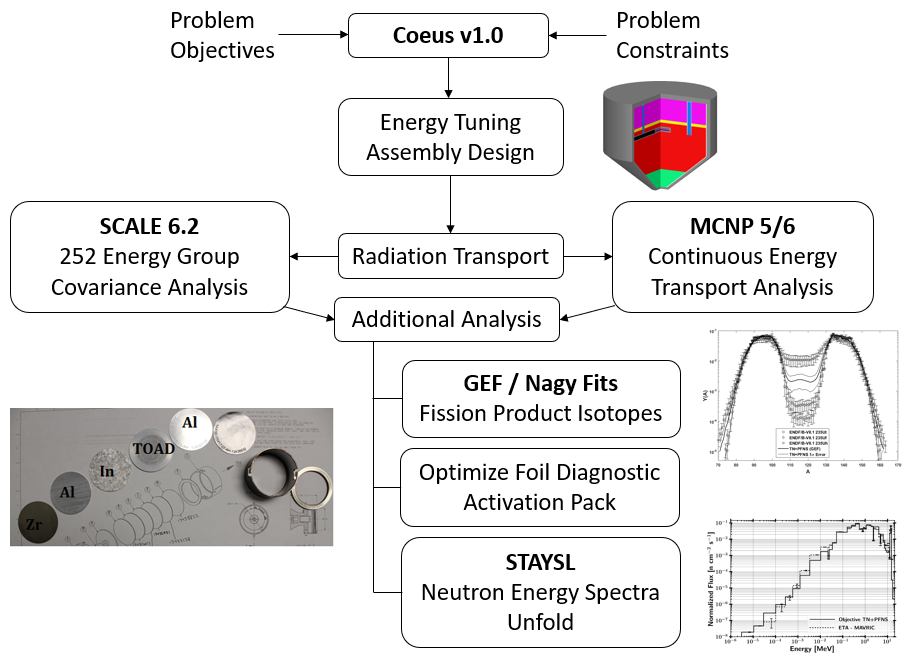
\includegraphics[width=\linewidth]{Figures/Chapter1/ETAFLOW1.png}
	\caption{Overview of the major research components for this work and how they are connected.}
	\label{fig:ETAFLOW}
\end{figure}

\section{Energy Tuning Assembly Design}

The spectral shaping problem is defined by the objectives and constraints. 
For this research, the problem objectives are the three spectra of fission product generation, enhanced fission product generation, and SPNS. % What are the 3 spectra of FP generation? The spectra used as objectives should be defined here. 
The problem constraints are based on the NIF source term and mechanical envelope. 
The input objectives and constraints are utilized in Coeus to produce a nearly-globally optimum solution for an ETA. 

\subsection{Enhanced Fission Debris Production Objective Spectrum}

Still gathering requirements

\subsection{Short Pulse Neutron Source Objective Spectrum}

Still gathering requirements 
%Unless we learn otherwise, I think the SPNS should use the same spectrum as the ETA II for enhanced fission.  We won't be able to field two devices anyways; two shots is questionable enough.

\subsection{NIF Constraints}

Still gathering requirements

\subsection{Coeus}

Describe any additional considerations in running Coeus here.

\section{Monte Carlo Transport}

Monte Carlo neutron transport will be performed with MCNP and SCALE for the 2019 ETA. 
The enhanced fission product ETA and ETA-SPNS will only be analyzed in MCNP due to time constraints. % we need shorthand for referring to ETA II.  Referring to ETA SPNS indicated a third ETA, which I don't think will be the case?
The point designs will modeled with MCNP and SCALE version 6.2 to perform neutron radiation transport. 
MCNP is used for continuous energy solution, while the SCALE's 252 group SAMPLER sequence around MAVRIC is used for group-wise covariance analysis. 
MAVRIC performs automated variance reduction techniques along with the traditional Monte Carlo transport calculations. 
MCNP versions 5 and 6 are both used depending on compatibility with surface source read (SSR) files generated by the NIF and LLNL. 
Utilizing two different radiation transport models increases the degree of confidence in the results. 
The radiation transport simulations provide results for the reaction rates for foil activation, neutron energy spectra, and temporal aspect of the neutron flux. 
% Why does the total source strength exceed 1 in SCALE?

\subsection{MCNP}

The SSR file was used to create sources representing the incident flux from the DT capsule and room return. 
The SSR file was initially created with the supporting equipment; however, no other experiments were involved. 
The SSR file contains two disk sources at the front and back of ETA and a cylindrical source on the sides of ETA. 
The surface fluxes were extracted using surface tallies in MCNP5, because the initial surface writing was performed with MCNP5. 
The geometry of the surface writing is shown in Figure \ref{fig:sursource}. 

\begin{figure}[ht]
	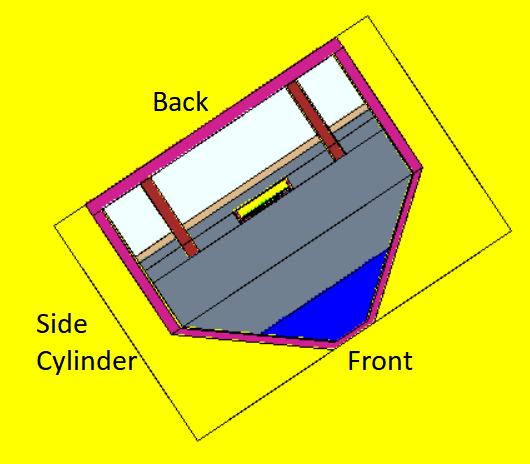
\includegraphics[width=\linewidth]{Figures/Chapter3/SurfacesSSR.png}
	\caption{Surfaces for NIF source SSR file.}
	\label{fig:sursource}
\end{figure}


The normalized probability distribution functions for the source locations are shown in Figure \ref{fig:RSSASpec}. 
The surface facing the source was approximated as a point source with the 14.03 MeV neutrons defining 1 source particle with a strength of 1.0063 source particles. 
The side cylindrical sources was approximated as four surrounding line sources at the same height which emitted at a solid angle to encapsulate the ETA. 
Ideally, the cylindrical source could be mapped over with a cylindrical source; however, the reference directions for emission in SCALE are in Cartesian coordination. 
The strength of the cylindrical source was $6.94*10^{-4}$ source particles split into the four line sources. 
The back disk source was modeled as a uniformly emitting disk source with a source strength of $9.44*10^{-4}$ source particles. 
The down-scattered neutrons are the "room return", which is a orders of magnitude below the actual source neutrons. 
Still, it is important to capture the impact of the room return, because the neutron cross-sections are in general larger at lower energy. 

\begin{figure}[ht]
	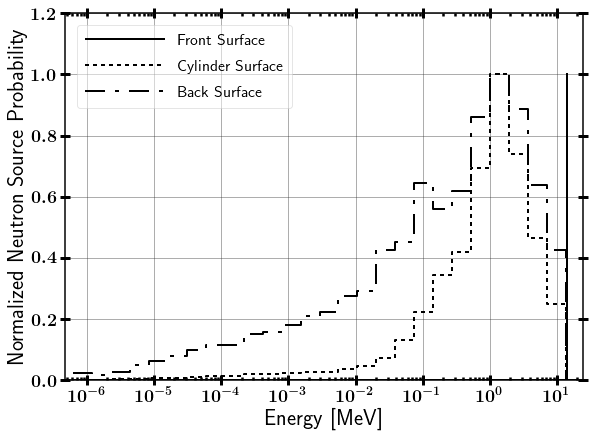
\includegraphics[width=\linewidth]{Figures/Chapter3/RSSA_Spectrum.png}
	\caption{Surfaces source probability distribution functions mapped to SCALE.}
	\label{fig:RSSASpec}
\end{figure}

The results from MCNP are used to benchmark a continuous energy solution in MAVRIC. 
Although it is not feasible to perfectly replicate the source distribution because there are many scattering angles crossing a surface in different directions, it is possible to get adequately close for the purpose of quantifying the impact of nuclear data covariance. 
The benchmarking of the mapping of MCNP to SCALE is performed by comparing the reactions in the foil pack. 
Two key aspects are important. 
First, the magnitude of the reactions nearly equivalent to about 1\%. % Include table/figure to illustrate?
Second, there is no pattern to the differences between SCALE and MCNP. 
Examples of important aspects that were looked for are that all the threshold or thermal reactions are not weighted heavily toward SCALE or MCNP. 

\subsection{SCALE SAMPLER Module}

SAMPLER is a SCALE module that enables analysis of nuclear data covariance. The unperturbed nuclear data is executed along with a user-defined number of samples. The samples have perturbed nuclear data based on the covariance. 
SAMPLER is distributed with 252 and 56 energy group structure libraries that have been created with evaluated data and approximated data. 
The covariance libraries are largely developed from ENDF/B-VII.1; however, additional information has been included from ENDF/B-VI, ENDF/B-VII.2 (proposed at the time), JENDL-4.0, and collaborative research between Brookhaven National Laboratory, Los Alamos National Laboratory, and Oak Ridge National Laboratory.
Finally, the nuclear data covariance libraries include information completed in the Working Party on International Nuclear Data Evaluation Cooperation Subgroup-26 \cite{SCALE}.

%- Aside 
%My plan only includes the nuclear data covariance for only the first ETA experiment. 
%I am interested in doing all of them; however, they do take a long time to get good results (especially at low energy bins). 
%In my research schedule I anticipate having to go through the whole process twice (something might be changed in the foil pack). 
%I might be able to get a second ETA analyzed with SAMPLER if things go as planned...
% If not, this is something we can push down the line.  I think it is of secondard importance, right now, to the primary objectives that you have outlined.  

SAMPLER requires on the order of hundreds samples to provide convergence of the responses \cite{SCALE}. The longer computational nature of SAMPLER runs is a constraint on the computational time available given the number of cores that can be used. Additionally, there are some issues with the SAMPLER sequence that have been addressed to ORNL, but may have an impact on the results. First, particles are sometimes "lost" in the simulation when traveling near parallel to a plane. It was determined that the lost particle effect was primarily due to the neutrons hitting a weight window boundary that is coincident with a plane in model. Second, some samples fail on execution when conducted on parallel. It is expected that the next large update to SCALE will fix these issues. 

\subsection{Comparison of Monte Carlo Neutron Transport Results}

The results from a Monte Carlo simulation often produce slightly different results when produced with different codes.The outputs are generally in more agreement for criticality continuations of critical assemblies and nuclear reactor analysis. 
It is important to gauge the impact to see how much variance is expected. 
Some of the differences are within the structure of the code itself, statistical error, different starting seeds, while others are based on the nuclear data that may be altered, or ultimately user error in setting up the geometry or source implementation. % Or differences in geometry and source implementation. I would consider those user error

Criticality in particular is a well-understood nuclear engineering problem that the nuclear data libraries are validated against. 
A study conducted on a high temperature pebble-bed reactor compared SCALE's version 6 CSAS6 code for criticality calculations to MCNP5's kcode\cite{Wang2014}. 
The results showed a difference for calculating $k_eff$ to be on the order of a few hundred percent mile ($10^{5}*(k{_eff}-1)/k$). 
This variance can easily be handled for reactor operations; however, this highlights that even well understood problems do have differences based on operating code. 
A similar study of a pebble bed reactor with varied geometry determined that the difference in MCNP to SCALE was near half a percent error\cite{Johnson2007}. %With a varied geometry?

A different study was conducted to determine the average gamma-ray doese outside of a spent nuclear fuel cask\cite{Chen2011}. 
The difference in dose rates between identically modeled SCALE and MCNP simulations varied as much as 27\%. 
Again, this shows that the less benchmarked studies can have larger errors which may be caused by user error. %It is an error, or variation in the modeled results? Obviously both cannot be right, but it isn't clear how similar the two were in terms of model. The report says they were identically modeled. My guess is this is user error

% The variance in the results for MCNP and SCALE performed in this work are not as large as here. %Huh?  I think this sentence is missing a few words
% The main source of difference is the mapping of the surface source from MCNP onto SCALE. Going to move this to the benchmarking SCALE to MCNP 

\subsection{Statistical Bootstrapping of SAMPLER Results}

SAMPLER is rooted in stochastic sampling of the nuclear
data covariance data \cite{SCALE}. Each sample in SAMPLER is a
perturbed set of nuclear data for the Monte Carlo simulation. It
is suggested that a typical number of samples is approximately
a few hundred \cite{SCALE}. SCALE is distributed with 1000 pre-built samples
for each available group structure.

The results of each of the sampled nuclear data libraries
with covariance can be combined using statistical bootstrapping.
Bootstrapping is a method to determine uncertainty in a
given dataset by using random sampling with replacement.
First, a sample generated is randomly selected between 0
and n samples. The 0 sample is the unperturbed nuclear data
result, while the 1 through n samples have perturbed nuclear
data. Next, the value of the corresponding sample number and
the relative uncertainty associated with the response are used
to sample a gaussian distribution. The gaussian distribution
individual bootstrap trial value selected based on the sampled
value and the uncertainty, given by the relative error. A diagram of the SAMPLER bootstrapping process is shown in Figure \ref{fig:boot}. 

% In general, figure titles that are full sentences and capture the takeaway are useful.  I can't say that I always follow this, but food for thought.
\begin{figure}[ht]
	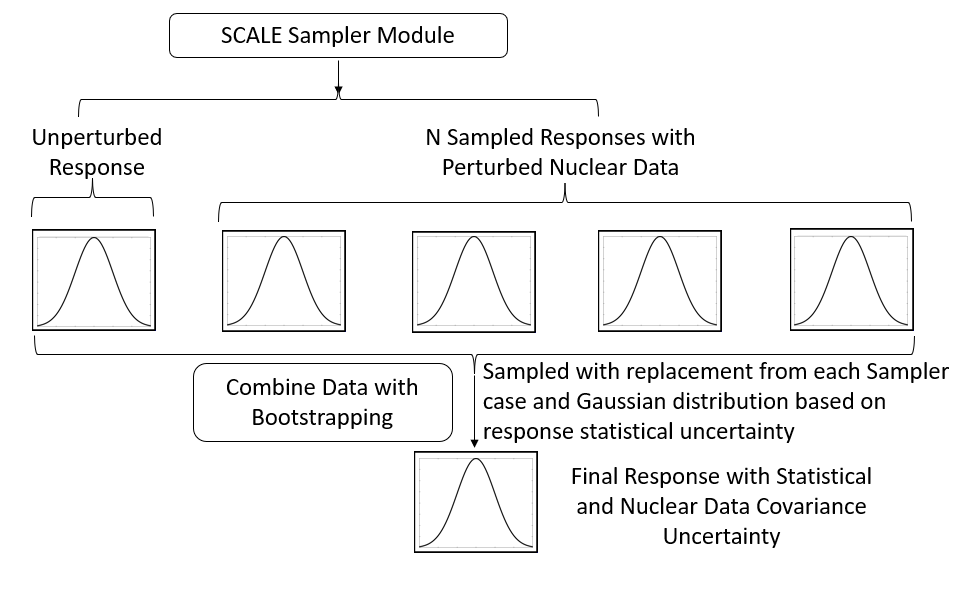
\includegraphics[width=\linewidth]{Figures/Chapter3/Bootstrapping.png}
	\caption{Bootstrapping  process utilized to combine SCALE SAMPLER results diagram}
	\label{fig:boot}
\end{figure}

Several python functions were built to parse and perform bootstrapping on the SAMPLER outputs.
First, the responses are read in, sorted, and stored. 
The stored data energy group strucutre is collapsed into a smaller group size to reduce uncertainty in the lower energy bins. 
The results are bootstrapped
20,000 times for each sample used in
SAMPLER to provide approximately 0.1\% convergence of the
bootstrapped relative error. The process of random sampling
is conducted with replacement to build up the sampled trials,
which are used to find the mean and standard deviation of the
bootstrap trial distribution.
The bootstrapped values are equivalent to a gaussian
distribution if the underlying data is Gaussian in shape. Bootstrapping
is useful to use here if a distribution of responses is
not perfectly Gaussian, or behaves in an unexpected manner.
The final value and relative uncertainty are used as the final result, which includes nuclear data covariance (a systematic uncertainty) and statistical uncertainty.
Other forms of systematic uncertainty will not be fully quantified. 
For example, the NIF source itself is a potential area of a large systematic uncertainty. 
The impact of perturbations to the source is explored separately in Section ???. 


\section{Activation Foils}

\subsection{Activation Foils Selection}

\ A foil pack designed to be placed in the ETA experimental cavity will be created to be able to successfully unfold the incident neutron spectra from the activation foils. 
The activation foils are selected with many important factors. 
The most notable aspects are the confidence in the nuclear data and energy range that the foils are activated. 

A study concluded, based on the energy groups ranging from 0.01 eV to 18 MeV, 
that Au, As, Cd, In, Ir, Er, Mn, Ni, Se, Sm, W, and Zn are suitable to fully 
cover the neutron energy spectrum \cite{Vagena2018b}. 
Key factors for the foils requirements included the cross-section, gamma emission, and half life. 
The half life was longer than 1 hr to enable off-site measurements, which is of interest for the experiment at the NIF. 

The foil pack used in the 2019 experiment will not have enough space to fit all of these foils. 
A preliminary set containing Au, In, Ni, W and Zn will be tested with the nuclear data activation rates to see if the foil pack is adequate. %Al?  Do these listed foils completely fill the volume, or is there one we can add based on the list above?  Mn maybe?

\subsection{Neutron Flux Unfolding with STAYSL}

\ The modeled foil activities are used with the underlying nuclear data to unfold the neutron spectrum using Pacific Northwest National Laboratory (PNNL) STAYSL. 
STAYSL relies on generalized least-squares spectral adjustment based on the chi-squared of the measured activities to determine the incident neutron flux \cite{Greenwood2016}. 
The nuclear data-covariance uncertainty is used as the activation uncertainty in the unfolding, which will provide a higher level of confidence in the spectral agreement. 
The true activation uncertainty will almost certainly be below that of the nuclear data covariance sampled values.

STAYSL's utilizes data from the IRDFF v1.05 library because of the increased level of benchmarking for dosimetry applications. 
Therefore, only reactions with data available in IRDFF are considered. 
Other reactions and foils are of interest; however, the foils included in STAYSL and IRDFF should be suitable. 


\section{Fission Product Generation}

GEF is utilized for developing the expected fission product isotopics. 
GEF is a Monte Carlo and theory based approach that incorporates experimental data to determine fission observables, such as fission products \cite{Schmidt2016}. 

GEF is applicable over a wide array of fissioning systems including isotopes with a atomic number from 80 to 112\cite{Schmidt2015}. 
Potential energy surfaces of the fission barrier of the fissioning system, theory, and adjustments based on empirical parameters have shown good predictive power\cite{Schmidt2014}. 
The modeled error can often be less than the experimental error. 
GEF incorporates covariance information and multi-chance fission, amongst many other attributes. 
Depending on the fissioning system, there are approximately 50 parameters that have been fit to align with experimental results. 
The inputs to the GEF model are the fissioning nucleus and energy of the incident particle. 

Nagy fits will also be used for comparison to GEF. 
An empirical fit to measured data not included in experiments is beneficial for comparison to GEF. % I don't understand this last sentence
% In general, I would say that the fission energy weighted empirical fits are likely to be more predictive than GEF, but data doesn't exist for all FPs of interest.

\section{Research Approach}
% This section is covered throughout and can be deleted to avoid repetition
Describe why you plan to apply your methodology. For example, prior
researchers may have implemented similar methods. On the other
hand, if your methods depart from standard practices or improve com-
monly used methods, you should state so.
Describe how you plan to implement your methodology.
{ For experimental work, you might discuss how you plan to evaluate
	your equipment and procedures.
	{ Computational work should include a discussion of methods that
		were developed by others, but that you'll implement, as well as
		the development of code that you plan to write.


\section{Uncertainty and Error Propagation}
% I would argue that this section and the error propogation section are common enough that they don't need to be explicitly stated and can be deleted. If you want to keep for completeness, that is ok too.
The calculated uncertainty in the results is driven by statistical uncertainty from Monte Carlo methods, $1/\sqrt{N}$. 
In addition to statistical uncertainty, the nuclear data covariance uncertainty provides one form systematic uncertainty. 

\subsection{Error Propagation}

Error propagation is important to some aspects of this analysis. 
One example where error propagation is required is when the 252 group structure from SAMPLER is collapsed. 
It is important to properly account for and track uncertainty through the entire problem. 

The propagation of uncertainty for a function ($q$) is the square root of the sum of squared uncertainty, ($\sigma_{x}$), of the variables, ($x, y, z,...$) multiplied by the the partial derivative of the function with respect to that variable\cite{Taylor}. 
The error propagation formula is given as

\begin{equation} \label{eq:errprop}
\sigma_{q} = \sqrt{(\dfrac{\partial q}{\partial x} \sigma_{x} )^2+(\dfrac{\partial q}{\partial y} \sigma_{y} )^2+(\dfrac{\partial q}{\partial z} \sigma_{z} )^2+...}
\end{equation}

\subsection{Chi-square Statistic and Interpretation}

The chi-square statistic, ($\chi^{2}$), is a useful tool for the interpretation of results to expected results. 
The reduced $\chi^{2}$, as used in the foil activation neutron flux unfolding, is \cite{Taylor}

\begin{equation} \label{eq:chi}
\dfrac{\chi^2}{DOF}= \dfrac{1}{DOF}\sum_{i=1}^{n} \; (\dfrac{\textit{observed value - expected value}}{\textit{observed standard deviation }})^2
\end{equation}

The degrees of freedom are defined based on the observed data points and parameters computed to fit the equation. 
The degrees of freedom is the number of measurements in one data set minus one for the case of comparing two data sets. 

The expected value for $\chi^{2}/DOF$ is unity if the calculated distribution is described by the expected distribution. 
$\chi^{2}/DOF$ much greater than one indicate that there is indeed a difference between the expected distribution and the observed. 
The  $\chi^{2}/DOF$ can be used to assess goodness of fit between two distributions. 

The p-value can be used to compare the results of the expected distribution to the calculated $\chi^{2}/DOF$. 
The p-value is the probability of finding a larger $\chi^{2}/DOF$, given the calculated result. 
The test of independence shows the probability of rejecting the null hypothesis, that the two distributions are the same. 
This probability is governed by the shape of the $\chi^{2}$ distribution.
An example of this is a $\chi^{2}$ of 16 with 4 degrees of freedom. 
The p-value from this is 0.003, which implies there is a strong significance of the results not being governed by the expected distribution. 
The null hypothesis is the rejected. 
A p-value of 0.05 is generally accepted as statistically significant; however, this can change depending on the field of study. 
Not rejecting the null hypothesis means the measured results are consistent with the expected; however, the $\chi^{2}$ test for independence cannot be used to prove the


\subsection{Systematic Uncertainties} \label{section1}

Systematic uncertainties, if known, are propogated exactly the same as error propagation formula. 
However, the systematic uncertainty is not known in many cases. 
The aspects of systematic uncertainty for the NIF experiments are discussed here. 

Geometric systematic uncertainty based on the positioning of the ETA, DT capsules, or components of ETA has the possibility to introduce systematic uncertainty. 
The NIF facility has rigid tolerances for positioning systems. 
It is assumed that the geometric uncertainty of this type is negligible.

A related uncertainty that may arise is the configuration of the NIF chamber. 
The planned configuration may not be the exact experiment performed, which ultimately requires that the analysis is repeated post-experiment if large perturbations are seen. 
An example of a change for the experiment might be another experiment in the room. 
A first order assessment looking at spheres of aluminum and lead simulating other experiments nearby showed that the total number of fissions for 2019 experiment can deviate by a few percent. 
All material in the chamber can cause backscattering and impact the solution to some degree. 

A source of systematic uncertainty is the neutron source itself, which is difficult to characterize completely. 
A scoping study was performed to analyze the impact of the source on the results. 
The interpretation of individual results will be presented later; however, it is important to understand to what extent the source may impact the solution. 
A 14.03 MeV point source is compared to a 10.75 keV plasma temperature Appelbe point source centered at 14.06 MeV, a 14.06 MeV  point source, the LLNL full NIF transported MCNP SSR, and the SCALE continuous energy results with the MCNP SSR mapped. 
The results for the comparison are shown in Figure \ref{fig:srccomp}. 

\begin{figure}[ht]
	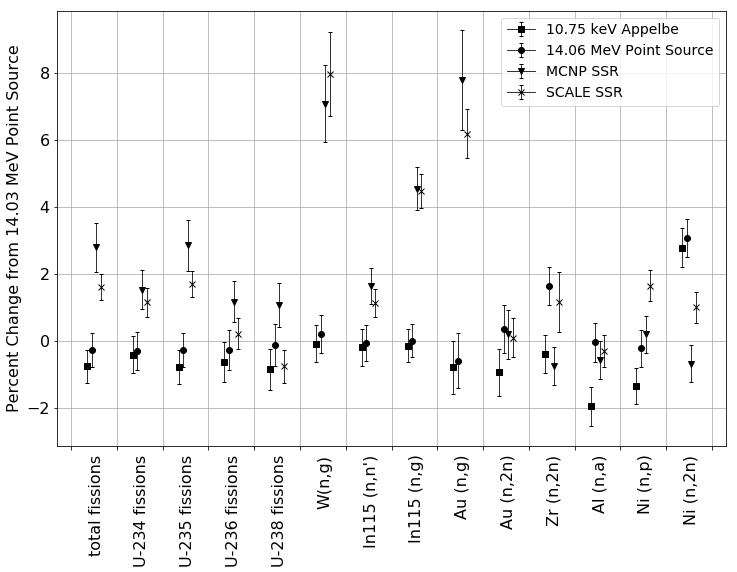
\includegraphics[width=\linewidth]{Figures/Chapter3/SourceComp.png}
	\caption[Comparison of results based on NIF source term. The statistical uncertainties of the underlying datasets are all less than 1\%]{Comparison of results based on NIF source term. The statistical uncertainties of the underlying datasets are all less than 1\%}
	\label{fig:srccomp}
\end{figure}
% I really like this plot - and despise it at the same time!  This looks to be a significant source of uncertainty.  This is worth bringing with us to LLNL (we should discuss at next research meeting everthing we should have printed and handy). 
% What is included in the error bars if the statistical uncertainty is < 1%?
 
The comparison shows a few key details. 
First, using higher energy source terms (Appelbe or 14.06 MeV) impacts the threshold reactions by as much as 2\%. 
The increase based on energy is expected as threshold generally increase with incident energy. 
Second, the thermal reactions increase substantially by including the room return and scattering back from the DIM. 
The down-scattered neutrons have lower energy and can contribute more to the total response. 
Last, the comparison between MCNP and SCALE SSR results is generally consistent. 
The deviations from the mean are not systematically distributed; for example not all MCNP threshold reactions are larger. 
 
